\chapter{Affine transformations of Gaussian RVs with application to parameter estimation}


\section{MVGs as a network of Linear Gaussians (LG)}

We often work with situations where an RV $\bm{x}$ is
affinely\footnote{This is also commonly referred to as a linear
Gaussian.}  transformed to an RV $\bm{y}$ i.e.
\begin{align*}
  \bm{y}=\bm{A}^{T}\bm{x}+\bm{c}+\bm{\nu},
\end{align*}
where
$\bm{x}\sim\mathcal{N}(\mu_{\bm{x}},\bm{\,\Sigma}_{\bm{xx}})$,
$\bm{c}$ is an offset vector and
$\bm{\nu}\sim\mathcal{N}(\bm{0},\,\bm{\Sigma}_{\bm{\nu\nu}})$.  As you
will see below, the joint $p(\bm{x},\bm{y})$ is also a Gaussian --
this proves useful in many situations. We can therefore reinterpret a
linear Gaussian description as a full joint Gaussian. The description
below is in terms of vector RVs, but the scalar case is easily
extracted by merely setting the dimensions of the vector in question,
to unity.

\subsection{From a linear Gaussian to a joint Gaussian}

Let us first consider $\bm{y}'=\bm{A}^{T}\bm{x}+\bm{c}$.
It is easy to show that
\[
\bm{y}'\sim\mathcal{N}(\bm{\mu_{\bm{y}'}=}\bm{A}^{T}\bm{\mu_{\bm{x}}}+\bm{c},\,\bm{\Sigma}_{\bm{y'y'}}=\bm{A}^{T}\Sigma_{\bm{xx}}\bm{A}).
\]
When we consider $\bm{x}$ and $\bm{y}'$ jointly (or conditionally),
the situation degenerates because the one determines the other. For
instance
$p(\bm{y'|}\bm{x)}=\delta(\bm{y'}-(\bm{A^{T}}\bm{x}+\bm{c}))$.  After
adding the noise term $\bm{\nu}$ (same dimension as $\bm{y}$), we are
in business again. The distribution for $\bm{y}$
now becomes:

\[
\bm{y}\sim\mathcal{N}(\bm{\mu_{\bm{y}}=}\bm{A}^{T}\bm{\mu_{\bm{x}}}+\bm{c},\,\bm{\Sigma}_{\bm{yy}}=\bm{A}^{T}\Sigma_{\bm{xx}}\bm{A}+\bm{\Sigma}_{\bm{\nu\nu}}).
\]


To specify the full joint $p(\bm{x},\bm{y})$ we still need
to determine the joint covariance $\bm{\Sigma}_{\bm{xy}}$:

\begin{align*}
\bm{\Sigma}_{\bm{xy}}= & \mathbb{E}[(\bm{x}-\mu_{\bm{x}})(\bm{y}-\mu_{\bm{y}})^{T}\\
= & \mathbb{E}[(\bm{x}-\mu_{\bm{x}})(\bm{\bm{A}^{T}\bm{x}}+\bm{\bm{c}}+\bm{\bm{\nu}}-(\bm{A}^{T}\bm{\mu_{\bm{x}}}+\bm{c}))^{T}]\\
= & \mathbb{E}[(\bm{x}-\mu_{\bm{x}})(\bm{A}^{T}(\bm{\bm{x}}-\bm{\mu_{\bm{x}}})+\bm{\bm{\nu}})^{T}]\\
= & \mathbb{E}[(\bm{x}-\mu_{\bm{x}})(\bm{(\bm{\bm{x}}-\bm{\mu_{\bm{x}}}){}^{T}A}+\bm{\bm{\nu}}^{T})]\\
= & \Sigma_{\bm{xx}}\bm{A}.
\end{align*}
The joint density therefore is:

\begin{equation}
\left[\begin{array}{c}
\bm{x}\\
\bm{y}
\end{array}\right]\sim\mathcal{N}\left(\left[\begin{array}{c}
\bm{\mu_{\bm{x}}}\\
\bm{\bm{A}^{T}\bm{\mu_{\bm{x}}}+\bm{c}}
\end{array}\right],\left[\begin{array}{cc}
\Sigma_{\bm{xx}} & \Sigma_{\bm{xx}}\bm{A}\\
\bm{A}^{T}\Sigma_{\bm{xx}}\hspace{5mm} & \bm{A}^{T}\Sigma_{\bm{xx}}\bm{A}+\bm{\Sigma}_{\bm{\nu\nu}}
\end{array}\right]\right).  \label{eq:linGaussToGauss}
\end{equation}

If we know the parameters
$(\mu_{\bm{x}},\bm{\,\Sigma}_{\bm{xx}},\,\bm{A} \text{ and } \bm{\Sigma}_{\bm{\nu\nu}})$ of an affine Gaussian specification, we
can use Eq \ref{eq:linGaussToGauss} to determine the corresponding
joint Gaussian distribution. Note, in contrast to earlier lectures, we
now think of $\bm{x}$ as an RV, not just a constant serving as parameter
of $\bm{y}$.


\paragraph{Example:}

We have a random variable $\mu\sim\mathcal{N}(0,1)$, and a second
random variable $x\sim\mathcal{N}(\mu,2)$ (i.e. $x$ is an RV centered
around whatever the value of RV $\mu$ is). Find and sketch their joint
distribution $p(x,\mu)$:

In this case we have $x=1\Mu+0+\nu$ with $\nu\sim\mathcal{N}(0,2)$.
Therefore from Eq.~\ref{eq:linGaussToGauss} we get the joint as:

\begin{align*}
\left[\begin{array}{c}
\mu\\
x
\end{array}\right]= & \mathcal{N}\left(\left[\begin{array}{c}
0\\
0
\end{array}\right],\left[\begin{array}{cc}
1 & 1\\
1 & 3
\end{array}\right]\right).
\end{align*}


For later use we also calculate the precision matrix

\begin{align*}
J= & \left[\begin{array}{cc}
1.5 & -0.5\\
-0.5 & 0.5
\end{array}\right].
\end{align*}


See Fig \ref{fig:bayesmeanest}(a) for a plot of the joint distribution.


\paragraph{Example:}

For the previous example, we observe%
\footnote{The true mean used to generate the $x_{i}$ values was $\mu=1.5$.%
} the following values

\begin{align*}
x_{1\ldots10}= & (-0.45,1.68,0.49,2.29,2.65,3.10,0.89,0.90,0.25,-0.04).
\end{align*}


From this, determine the sequential (i.e. after the first observation,
then after the first two observations, etc.) ML, MAP and Bayesian
estimates for the distribution of $p(x|x_{1\ldots N_{i}})$ with
$N_{i}=1\ldots10$.

a) The ML estimate is simply the arithmetic mean of the observations:

\begin{align*}
\mu_{\mbox{MLE}}(x_{1\ldots N_{i}})= & \frac{\sum_{n=1}^{N_{i}}x_{n}}{N_{i}}.
\end{align*}


Sequentially (i.e. as we use more and more data) this gives the estimates:

\begin{align*}
\mu_{\mbox{MLE}}(x_{1\ldots N_{i}})= & (-0.450,0.615,0.573,1.003,1.332,1.627,1.521,1.444,1.311,1.176),
\end{align*}
with $N_i = 1,2, \ldots , 10$.

b) The MAP estimate of the mean is the $\mu$ that maximises

\begin{align*}
p(\mu)\prod_{i}p(x_{i}|\mu)= & \exp\left[-\frac{\mu^{2}}{2}-\sum_{i}\frac{(x_{i}-\mu)^{2}}{4}\right].
\end{align*}


Taking the log and setting the derivative wrt $\mu$ equal to zero
gives:

\begin{align*}
\mu_{\mbox{MAP}}(x_{1\ldots N_{i}})= & \frac{\sum_{n=1}^{N_{i}}x_{n}}{N_{i}+2}.
\end{align*}


In effect it is as if we had, in this case, two 'phantom' observations,
both placed at the mean of the prior i.e. at zero. Note that that
the variance of the prior dictates the number of 'phantom' observations.
The sequence of estimates (with growing $N_i)$ now changes to:

\begin{align*}
\mu_{\mbox{MAP}}(x_{1\ldots N_{i}})= & (-0.150,0.308,0.344,0.668,0.951,1.220,1.183,1.155,1.072,0.980).
\end{align*}


For both ML and MAP we work with point estimates, resulting in a distribution
for $x$ given by:

\begin{align*}
p(x|x_{1\ldots N_{i}})= & \mathcal{N}(\mu_{\mbox{est}}(x_{1\ldots N_{i}}),2).
\end{align*}


c) For the Bayesian estimate, lets start out with the graphical model
that describes $p(\mu,x|x_{1\ldots N})$:

\begin{figure}[!h]
  \hfill\begin{centering}
    \parbox{0.4\textwidth}{
      \centering
        \psfragfig*[height=6cm,crop=pdfcrop]{bayesianmean_BN} \\
        %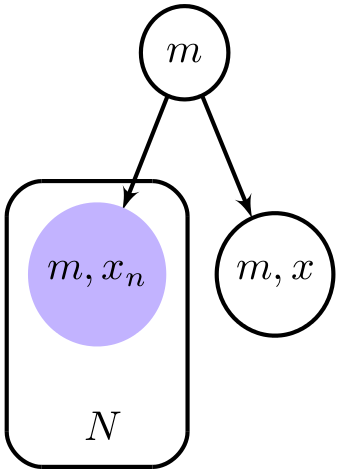
\includegraphics[width=3cm]{bayesianmean_BN} \\
      (a) Represented as a Bayes net.
    }
  \end{centering}\hfill
  %%%%%%%%%%%%%%
  \begin{centering}
    \parbox{0.4\textwidth}{ \centering
      \psfragfig*[height=6cm,crop=pdfcrop]{bayesianmean_CG} \\
      %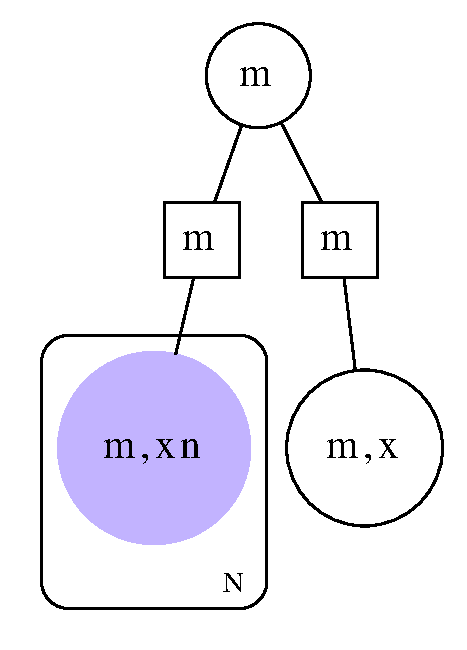
\includegraphics[width=3cm]{bayesianmean_CG}\\
 (b) Represented as a cluster graph ($\mu$ is unobserved).
}
  \end{centering} \hfill
  %%%%%%%%%%%%%%
\caption{Bayesian estimation of a mean given known covariance and
  prior. We include the extra unobserved $x$ because we are interested
  in the joint distribution of $x$ and $\mu$.}
  \label{fig:lingaus_graphs}
\end{figure}


Note from Fig. \ref{fig:lingaus_graphs}(a) that the joint
\begin{align*}
  p(\mu,x,x_{1\ldots N}) &= p(\mu) p(x|\mu)p(x_{n}|\mu).
\end{align*}
To keep things simple, we will use them in canonical form.

For the prior $p(\mu)$ the canonical parameters are:

\begin{align*}
\bm{K}_{\mu}= & \left[\begin{array}{cc}
1 & 0\\
0 & 0
\end{array}\right]\mbox{ and }\\
\bm{h}_{\mu}= & \left[\begin{array}{c}
0\\
0
\end{array}\right].
\end{align*}
The joint $p(\mu,x)$ we obtained in the previous example:

\begin{align*}
\bm{K}_{\mu,x}= & \left[\begin{array}{cc}
1.5 & -0.5\\
-0.5 & 0.5
\end{array}\right]\mbox{ and }\\
\bm{h}_{\mu,x}= & \bm{0}.
\end{align*}

With the conditional distributions of the form $p(x|\mu)$ we have to
be somewhat careful -- normally when we want a conditional
distribution we simply observe the value in the joint distribution and
that is it. However, in this case that will leave us with
$p(\mu|x_{n})$ which is not what we want. The problem arises because
the observed RV $x_{n}$ now is to the \emph{left} of the condition
bar, not in its usual place to the right of it. Either we have to
consider $\exp\left[-\sum_{n}\frac{(x_{n}-\mu)^{2}}{4}\right]$ as a
function of $\mu$ with known $x_{n}$'s, or we can equivalently
determine it via $p(x_{n}|\mu)=\frac{p(\mu,x)}{p(\mu)}.$ Using
canonical form division we get the corresponding canonical parameters
as:

\begin{align*}
\bm{K}_{x|\mu}= & \left[\begin{array}{cc}
0.5 & -0.5\\
-0.5 & 0.5
\end{array}\right]\mbox{ and }\\
\bm{h}_{x|\mu}= & \bm{0}.
\end{align*}


Note that $\bm{K}_{x|\mu}$ is singular, this should not be a surprise
since it describes a one-dimensional function. When we now observe a
particular $x_{n}$ this becomes (see Koller for the equations for
canonical form reduction):

\begin{align*}
\bm{K}_{x_{n}|\mu}= & \left[\begin{array}{cc}
0.5 & 0\\
0 & 0
\end{array}\right]\mbox{ and }\\
\bm{h}_{x_{n}|\mu}= & \left[\begin{array}{c}
0.5x_{n}\\
0
\end{array}\right].
\end{align*}

The canonical form of our full\footnote{Something interesting is
going on here with the inclusion of the $p(x|\mu)$ term and its effect
via $\bm{K}_{x|\mu}$. It does change the posterior very slightly --
only by omitting it do we get a posterior with its maximum exactly at
the MAP estimate point.} joint $p(\mu,x|x_{1\ldots N})$ is now given
by:

\begin{align*}
\bm{K}_{\mu,x|x_{1\dots N_{i}}}= & \bm{K}_{\mu}+\bm{K}_{x|\mu}+\sum_{n=1}^{N_{i}}\bm{K}_{x_{n}|\mu},\\
= & \left[\begin{array}{cc}
1.5+0.5N_{i} & -0.5\\
-0.5 & 0.5
\end{array}\right]\mbox{ and }\\
h_{\mu,x|x_{1\dots N_{i}}}= & \bm{h}_{\mu}+\bm{h}_{x|\mu}+\sum_{n=1}^{N_{i}}\bm{h}_{x_{n}|\mu}\\
= & \left[\begin{array}{c}
0.5\sum_{n=1}^{N_{i}}x_{n}\\
0
\end{array}\right].
\end{align*}


\begin{figure}
  \begin{centering}
  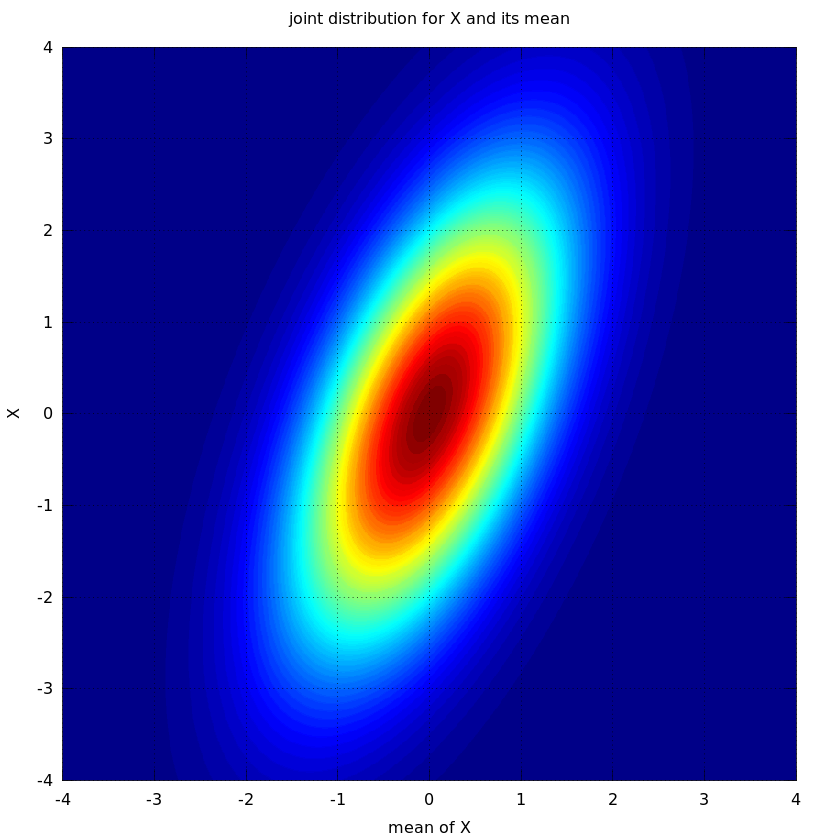
\includegraphics[width=6cm]{bayesmean0}\\
  (a) The joint $p(\mu,x)$. The correlation between $\Mu$ and $x$ is
  clear, vertical cuts shifts the conditional distribution $p(x|\mu)$.
  \end{centering}

  \begin{centering}
  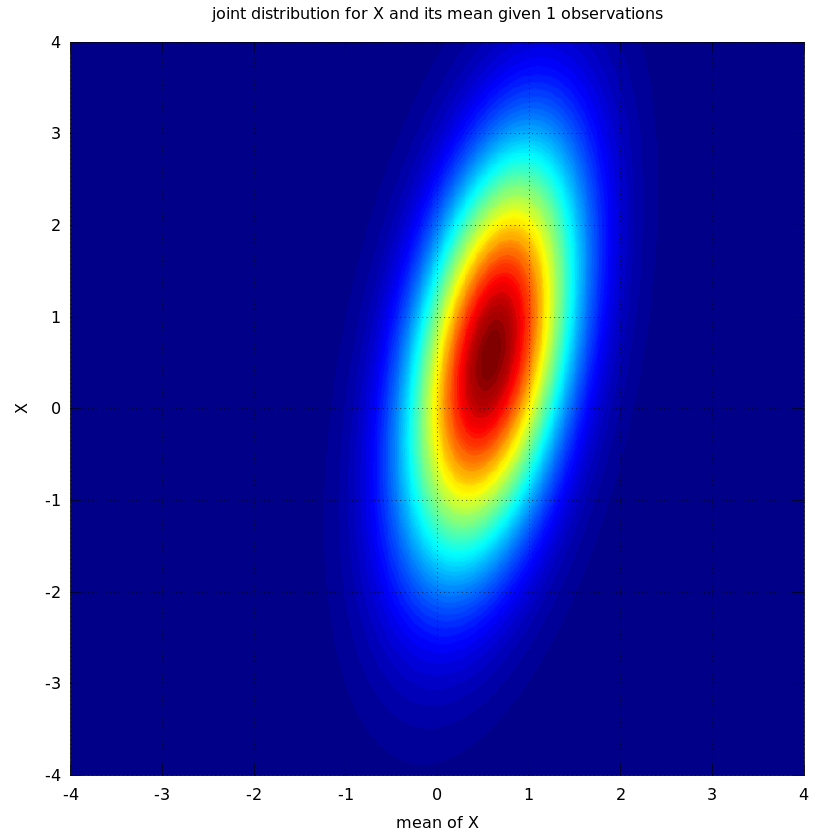
\includegraphics[width=6cm]{bayesmean1}\\
  (b) The joint $p(\mu,x|x_{1})$ (i.e. after taking one observation into
  account). A marked but controlled shift away from the prior, is evident.
  \end{centering}

  \begin{centering}
  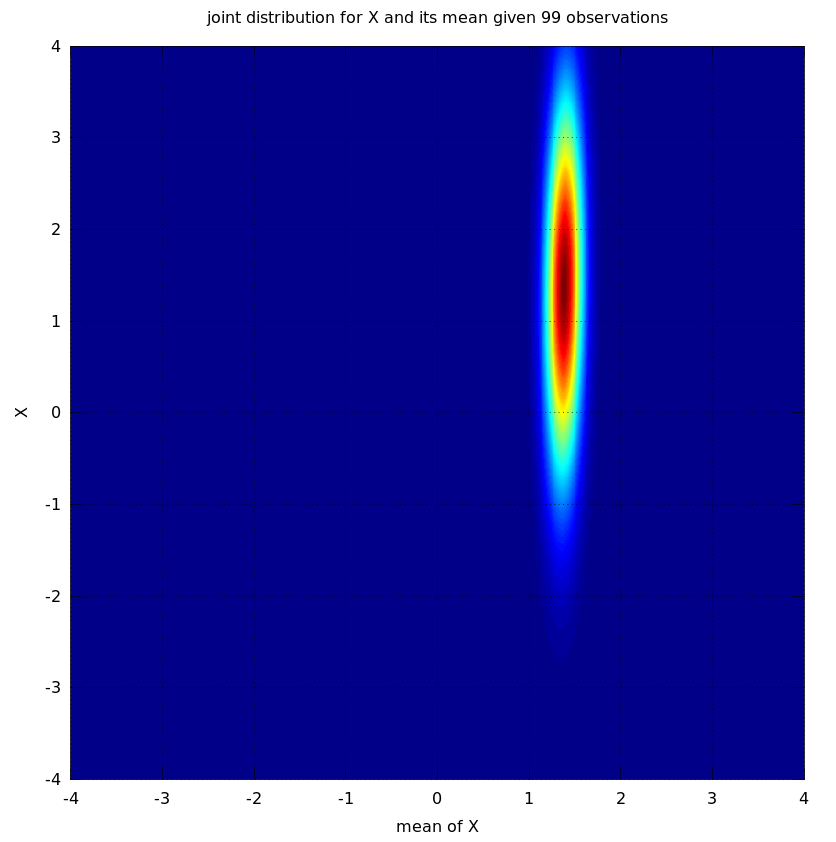
\includegraphics[width=6cm]{bayesmean99}\\
  (c) The joint $p(\mu,x|x_{1\ldots99})$ (i.e. after 99 observations).
  The estimate now lies quite close to the true underlying value (which
  was 1.5).
  \end{centering}

\caption{Bayesian estimation of the mean $\mu$ of RV $x$.}
\label{fig:bayesmeanest}
\end{figure}


Note how the inclusion of $\bm{K}_{\mu}$ on the right hand side
reverts the precision matrix to a non-singular
state. Fig. \ref{fig:bayesmeanest} shows how observing more and more
$x_{n}$ values refines our knowledge about the distribution of $\mu$.

\paragraph{Reflection:}

A subtly beautiful thing, worthwhile to reflect on, has happened here.

With the ML and MAP estimates, we designed a cost function (based
on the likelihood and prior information) and framed the problem as
estimating the \emph{single parameter point} that minimises the chosen
cost function. To do this we had to solve an \emph{optimisation} problem
-- this was quite easy for the Gaussians (it had a closed form), but
could be extremely hard for some other distributions. But if we substitute
for another set of observations, it will be different. And our point
estimate has no way to characterise this variability.

The central hard things to do in Bayesian estimates, are marginalisation
and observation. For the Gaussian the solution to these is provided
via the canonical form. We now change the problem from that of estimating
a parameter point, to estimating the \emph{distribution} of the parameters
given our prior knowledge and observations. We find this distribution,
not by optimising, but by doing inference, i.e. some form of message
passing in a graphical model. \emph{Learning now becomes inference!}
For this specific case the resultant PGM has a tree structure and
is therefore exactly solvable. In general it will have a graph structure
and we can approximately solve it using loopy belief propagation.
It can be shown \cite{Barber2012} that this is equivalent to approximate
the Bayesian estimate via variational inference\cite{MacKay2003}.
This generalising view of representing parameters by a distribution
instead of a point, makes the system much more resistant to overfitting.

In this specific case, our observations were also independent given
the parameters. We can therefore also cast this into a sequential
Bayesian estimation where we combine the prior and the first observation
to estimate a posterior distribution for the parameters (a very simple
PGM). This posterior then becomes the prior for the second observation
etc., we keep on iterating the process as we acquire more and more
information.


\subsection{From a joint Gaussian to a linear Gaussian}

It is also useful to reduce a full Gaussian description to linear
Gaussian. If we have the full Gaussian distribution available as:

\[
\left[\begin{array}{c}
\mathbf{X}\\
\mathbf{Y}
\end{array}\right]\sim\mathcal{N}\left(\left[\begin{array}{c}
\mathbf{\mu_{\mathbf{X}}}\\
\mathbf{\mu_{\mathbf{Y}}}
\end{array}\right],\left[\begin{array}{cc}
\Sigma_{\mathbf{XX}} & \Sigma_{\mathbf{XY}}\\
\Sigma_{\mathbf{YX}}=\Sigma_{\mathbf{XY}}^{T}\hspace{5mm} & \Sigma_{\mathbf{YY}}
\end{array}\right]\right),
\]
 we can find the corresponding linear Gaussian parameters as follows:

Firstly, $\mu_{\mathbf{X}}$ and $\Sigma_{\mathbf{XX}}$ are directly
known from the full covariance description. We can determine $\mathbf{A}$
from the covariance term:

\begin{align}
\Sigma_{\mathbf{XY}}= & \Sigma_{\mathbf{XX}}\mathbf{A}\nonumber \\
\therefore\mathbf{A}= & \Sigma_{\mathbf{XX}}^{-1}\Sigma_{\mathbf{XY}}.
\end{align}


With that known, $\mathbf{c}$ is easily solved by comparing the means:

\begin{equation}
\mathbf{c}=\mu_{\mathbf{Y}}-\mathbf{A}^{T}\mathbf{\mu_{\mathbf{X}}}.
\end{equation}
Finally we solve the noise covariance as:

\begin{align}
\mathbf{\Sigma}_{\mathbf{NN}}= & \Sigma_{\mathbf{YY}}-\mathbf{A}^{T}\Sigma_{\mathbf{XX}}\mathbf{A}\nonumber \\
= & \Sigma_{\mathbf{YY}}-\mathbf{A}^{T}\Sigma_{\mathbf{XY}}.
\end{align}



\subsection{Ponderings on generalising to more dependencies }

NOTE: You can easily skip this bit, I was just exploring for a moment
to see where it might lead. And my conclusion is ``nowhere special''.

Let us now generalise to the case where $\mathbf{Y}$ is dependent
on multiple $\mathbf{X}_{i}'s$ i.e.

\[
\mathbf{Y}=\mathbf{\sum_{i=1}^{N}A_{i}}^{T}\mathbf{X_{i}}+\mathbf{c_{i}}+\mathbf{N_{i}},
\]
with each $\mathbf{X_{i}}\sim\mathcal{N}(\mu_{i},\mathbf{\,\Sigma}_{ii})$
and $\mathbf{N_{i}}\sim\mathcal{N}(\mathbf{0},\, R_{ii})$ distinct
and independent of the others.

We can visualize this as a Bayes net, shown in Fig \ref{fig:lingauss_bn}.
Note that, with $\mathbf{Y}$ unobserved, all the $\mathbf{X}_{i}$'s
are statistically independent from each other. However, when $\mathbf{Y}$
is known, they all become conditionally dependent on each other. I.e.
the moralizing process involved when converting from a Bayes-net to
a Markov-random-field, will tie all these variables into one (large)
cluster/clique, irrespective of whether $\mathbf{Y}$ was observed
or not. These general independencies unfortunately does not necessarily
imply conditional independencies - the information might still be
dense in spite of a very sparse covariance matrix.

\begin{figure}
\noindent \begin{centering}
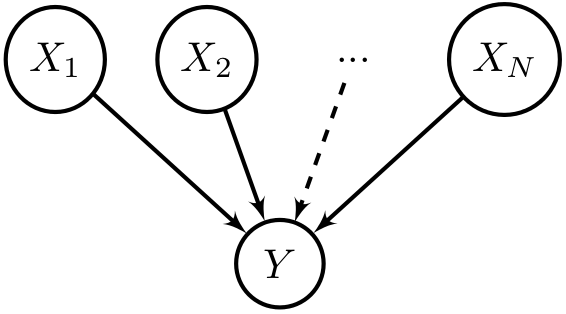
\includegraphics[height=3cm]{lingauss_bn}
\par\end{centering}

\caption{General linear Gaussian.}
\label{fig:lingauss_bn}
\end{figure}


The full Gaussian describing this situation is given by:

\begin{equation}
\left[\begin{array}{c}
\begin{array}{c}
\mathbf{X}_{1}\\
\vdots\\
\vdots\\
\mathbf{X}_{N}\\
\mathbf{Y}
\end{array}\end{array}\right]\sim\mathcal{N}\left(\left[\begin{array}{c}
\mathbf{\mu}_{1}\\
\vdots\\
\vdots\\
\mathbf{\mu}_{N}\\
\mathbf{\mathbf{\sum_{i=1}^{N}A_{i}}^{T}\mathbf{\mu_{i}}+\mathbf{c_{i}}}
\end{array}\right],\left[\begin{array}{ccccc}
\Sigma_{11} & \mathbf{0} & \hdots & \mathbf{0} & \Sigma_{11}\mathbf{A}_{1}\\
\mathbf{0} & \ddots & \ddots & \vdots & \vdots\\
\vdots & \ddots & \ddots & \mathbf{0} & \vdots\\
\mathbf{0} & \hdots & \mathbf{0} & \Sigma_{NN} & \Sigma_{NN}\mathbf{A}_{N}\\
\mathbf{A}_{1}^{T}\Sigma_{11} & \hdots & \hdots & \mathbf{A}_{N}^{T}\Sigma_{NN} & \hspace{5mm}\sum_{i=1}^{N}\mathbf{A}_{i}^{T}\Sigma_{ii}\mathbf{A}_{i}+\mathbf{R}_{ii}
\end{array}\right]\right).
\end{equation}


Note the blocks of zeros in the covariance matrix, these indicates
that the corresponding random vectors are independent \emph{if $\mathbf{Y}$}
is not known. The equations for determining the linear Gaussian parameters
from the full covariance description now becomes:

\begin{eqnarray}
\mathbf{A}_{i} & = & \Sigma_{ii}^{-1}\Sigma_{i\mathbf{Y}},\\
\sum_{i=1}^{N}\mathbf{c}_{i} & = & \mu_{\mathbf{Y}}-\sum_{i=1}^{N}\mathbf{A}_{i}^{T}\mathbf{\mu}_{i},\mbox{ and}\\
\sum_{i=1}^{N}\mathbf{R}_{ii} & = & \Sigma_{\mathbf{YY}}-\sum_{i=1}^{N}\mathbf{A}_{i}^{T}\Sigma_{i\mathbf{Y}}.
\end{eqnarray}


Note that with both $\mathbf{c}_{i}$ and $\mathbf{R}_{ii}$ we have
some extra freedom. However, the covariances must still remain symmetric
and positive definite.


\section{MVGs as a network of bi-variate Gaussians (BVGs)}


\subsection{The general idea}

Representing a multi-variate Gaussian as a network of two-dimensional
Gaussians can be very useful. Amongst others this simplifies the required
operations such as inversion etc greatly. The likely price to pay
is that the resultant structure will be loopy. Is this doable? The
short answer is a qualified yes, Koller \cite[Section 14.2.3]{Koller2009}
shows how. However, her solution has a few aspects that might not
work well with our EMDW implementation:
\begin{itemize}
\item The solution is explicitly framed as a factor graph whereas we prefer
to work with cluster graphs. Of course, with variable pairs, the graph
will always implicitly end up as being a factor graph but, instead
of dictating it from the outside, we prefer EMDW to do the configuration
automatically. In the interaction with other MVGs, things might go
wrong.
\item She breaks the graph up into a number of pairwise factors, and a number
of single factors. However, the pairwise factors can not stand on
their own legs, they \emph{must }receive their messages from the single
factors before they are able to send out their own messages. This
just might cause trouble in a loopy system if we do not explicitly
specify the message passing order beforehand -- I'm also unsure as
to how well this will work with an initial vacuous canonical form.
\end{itemize}
The approach we develop here directly models the MVG as a network
of BVG's where each BVG is a fully functional Gaussian distribution.
Fig. \ref{fig:gaussianpairs_cg} illustrates the resulting structure
as a cluster graph of BVGs. The illustration is for the five-dimensional
case, but how to extend it to arbitrary dimensions is clear. Such
a network will consist of $\frac{D(D-1)}{2}$ BVG nodes, with $D$
the number of variables represented by the MVG. Although we show the
full connected cluster graph structure (obeying the RIP property),
in general we will not concern ourselves with linking the BVG factors
-- in the EMDW system that is handled automatically by the code. If
the MVG information matrix $J$ has zeros in some locations, the corresponding
BVG terms disappear, thereby simplifying the cluster graph.

\begin{figure}
\noindent \begin{centering}
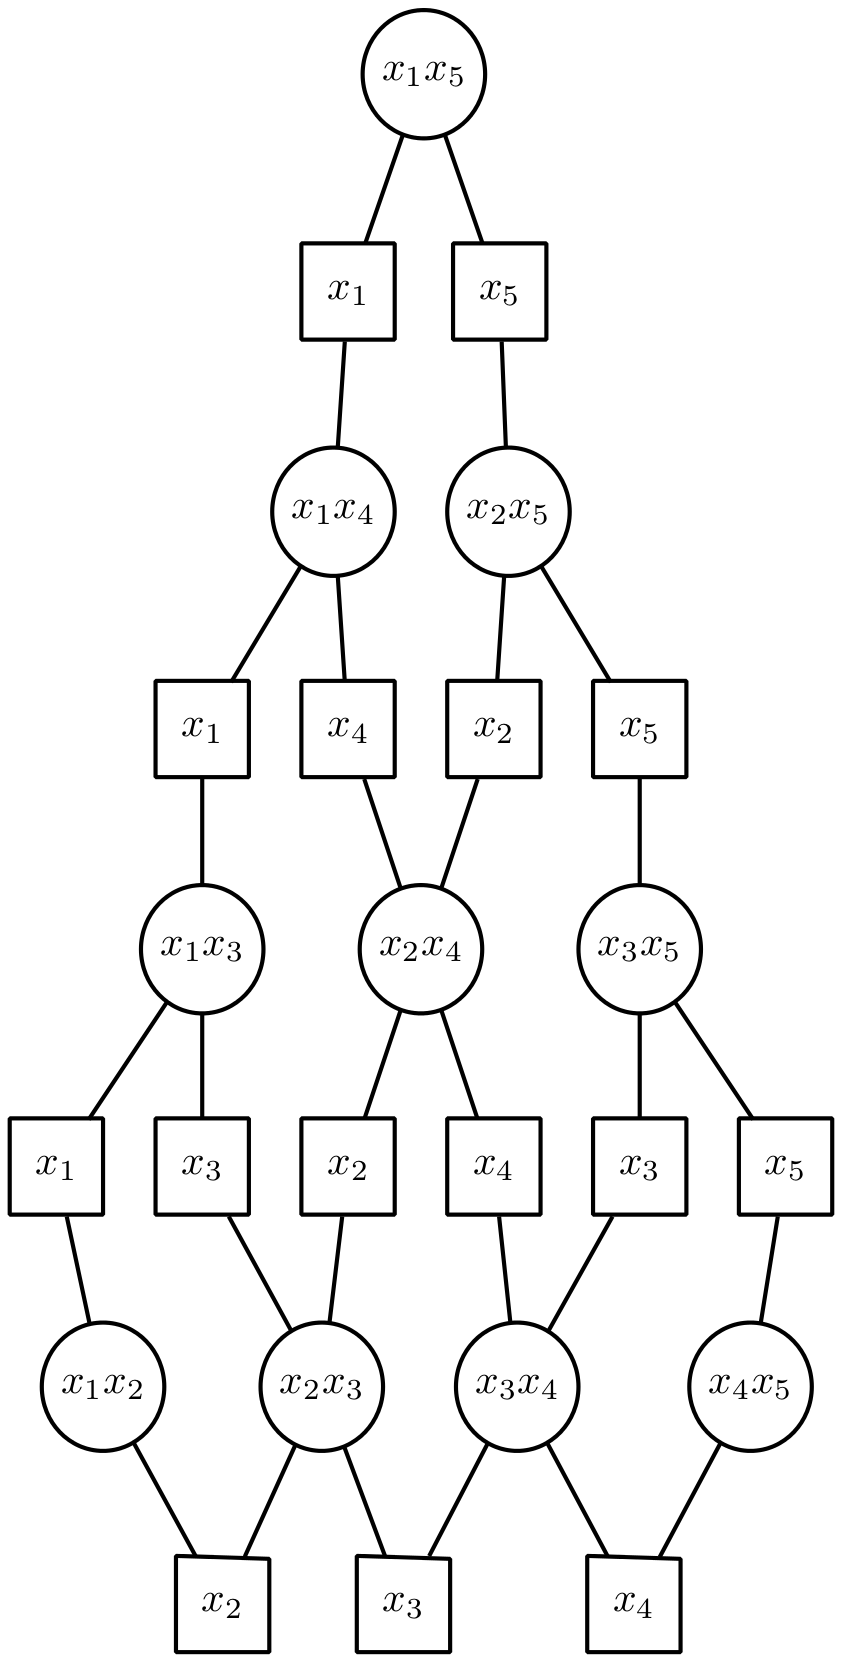
\includegraphics[height=10cm]{gaussian_pairs}
\par\end{centering}

\caption{Representing a multi-variate Gaussian on $X_{1}\hdots X_{5}$ as a
cluster graph with pairwise clusters.}
\label{fig:gaussianpairs_cg}
\end{figure}


We will find that such a structure is indeed adequate for representing
a general MVG. However, the BVGs are not uniquely specified, and the
requirement that their covariance matrices be symmetric and positive
definite, will introduce a constrained optimization as a subtask in
configuring them. Fortunately this is only necessary when initially
setting up the network, during the subsequent inference procedure
the message passing do not change the scope of the the BVGs and processing
is quite efficient.

Since both BVGs and 1VGs are just a special case of the MVG, there
also should be no limitation on combining them in a network.

To fix ideas, we are below first going to investigate the three-dimensional
case, and after that generalise to the $d$-dimensional case.


\subsection{Representing a three-dim Gaussian as three two-dim Gaussians \label{sub:Representing-a-three-dim}}


\subsubsection{From a product of three BVGs to an three-dim MVG}

Consider the product of generic canonical forms $\mathcal{C}(x,y;K_{1,2},\mathbf{h}_{1,2})\mathcal{C}(y,z;K_{2,3},\mathbf{h}_{2,3})\mathcal{C}(x,z;K_{1,3},\mathbf{h}_{1,3})$.
The identifying subscripts were chosen with some advance knowledge,
for now simply accept them as such. It covers all the pairwise connections
if we were to work with three RVs $X,Y\mbox{ and }Z$. We first have
to extend the three scopes to a common one. The information matrices
then become:

\begin{align*}
K_{1,2}= & \left[\begin{array}{ccc}
K_{1,2}^{x,x} & K_{1,2}^{x,y} & 0\\
K_{1,2}^{y,x} & K_{1,2}^{y,y} & 0\\
0 & 0 & 0
\end{array}\right],\\
K_{2,3}= & \left[\begin{array}{ccc}
0 & 0 & 0\\
0 & K_{2,3}^{y,y} & K_{2,3}^{y,z}\\
0 & K_{2,3}^{z,y} & K_{2,3}^{z,z}
\end{array}\right],\\
K_{1,3}= & \left[\begin{array}{ccc}
K_{1,3}^{x,x} & 0 & K_{1,3}^{x,z}\\
0 & 0 & 0\\
K_{1,3}^{z,x} & 0 & K_{1,3}^{z,z}
\end{array}\right].
\end{align*}


The potential vectors become:

\begin{align*}
\mathbf{h}_{1,2}= & \left[\begin{array}{c}
h_{1,2}^{x}\\
h_{1,2}^{y}\\
0
\end{array}\right],\\
\mathbf{h}_{2,3}= & \left[\begin{array}{c}
0\\
h_{2,3}^{y}\\
h_{2,3}^{z}
\end{array}\right],\\
\mathbf{h}_{1,3}= & \left[\begin{array}{c}
h_{1,3}^{x}\\
0\\
h_{1,3}^{z}
\end{array}\right].
\end{align*}
Since the $g$'s are scalar, they remain unchanged. Then we can apply
the rule for the product of canonical forms (Eq \ref{eq:cfprod})
to obtain (we identify it with an $\mbox{MVG}$ subscript in anticipation
of its later use):

\begin{align}
K_{\mbox{\mbox{MVG}}}= & \left[\begin{array}{ccc}
K_{1,3}^{x,x}+K_{1,2}^{x,x}\hspace{5mm} & K_{1,2}^{x,y} & K_{1,3}^{x,z}\\
K_{1,2}^{y,x} & K_{1,2}^{y,y}+K_{2,3}^{y,y}\hspace{5mm} & K_{2,3}^{y,z}\\
K_{1,3}^{z,x} & K_{2,3}^{z,y} & K_{2,3}^{z,z}+K_{1,3}^{z,z}
\end{array}\right],\\
\mathbf{h}_{\mbox{\mbox{MVG}}}= & \left[\begin{array}{c}
h_{1,3}^{x}+h_{1,2}^{x}\\
h_{1,2}^{y}+h_{2,3}^{y}\\
h_{2,3}^{z}+h_{1,3}^{z}
\end{array}\right],\mbox{ and }
\end{align}


This then shows the relationship between the parameters of the three
two-dim Gaussians, and that of their product.
\begin{itemize}
\item Note the one-to-one relationship of the off-diagonal terms of the
MVG to the off-diagonal terms of the BVGs -- they uniquely specify
each other.
\item However, from the summations in the diagonal terms of $K_{\mbox{MVG}}$
it is clear that the diagonal terms of the BVG information matrices
are not uniquely determined. However, this allocation will also have
to take into account that these covariances \emph{must }be symmetric
and positive definite.
\item In allocating values to $\mathbf{h}_{i}$ we also have some freedom
-- in this case there does not seem do be any special restrictions.
It should be safe to, for instance, simply split them equally.
\end{itemize}

\subsubsection{Equivalency of an MVG to a product of BVGs}

Clearly the product of BVGs is an MVG. Is this fully generic in the
sense that we can represent any MVG as the product of BVGs? Intuitively
one would think so, but unfortunately this is not so.


\paragraph{Definitions: Attractive and Diagonally Dominant:}

Symmetric matrices that are either attractive or diagonally dominant,
are guaranteed to be positive definite \cite[p 256]{Koller2009}. However,
although \emph{sufficient}, these conditions are not \emph{necessary}
for positive definiteness.
\begin{itemize}
\item According to Koller a matrix $J$ is said%
\footnote{This does not make sense to me. However, the partial correlation between
$i$ and $j$ is $\frac{-J_{i,j}}{\sqrt{J_{i,i}J_{j,j}}}$ and I presume
its absolute value should be less than one. My guess is what was intended
is: $|J_{i,j}|<\sqrt{J_{i,i}J_{j,j}}$. In similar vein I wonder if
for a covariance matrix a useful test for validity would be that the
magnitude of all correlation coefficients $|\rho_{i,j}|<1$ i.e. $|\sigma_{i,j}|<\sigma_{i}\sigma_{j}$.%
} to be attractive if, for all $i\neq j$: $-J_{i,j}\geq\sqrt{J_{i,i}J_{j,j}}$.
\item A matrix $J$ is said to be diagonally dominant if, for all%
\footnote{Personally I suspect that it will still be guarranteed positive definite
if we also allow equality for all but one of the diagonals.%
} $i$: $\sum_{j\neq i}|J_{i,j}|<J_{i,i}$.
\end{itemize}
Let us now consider the following information matrix (still from Koller):

\begin{align*}
J= & \left[\begin{array}{ccc}
1 & 0.6 & 0.6\\
0.6 & 1 & 0.6\\
0.6 & 0.6 & 1
\end{array}\right].
\end{align*}


Although neither diagonally dominant nor attractive, this matrix still
is positive definite with eigenvalues $\{0.4,0.4,2.2\}$ and $|J|=0.352$.
It therefore is a valid MVG information matrix. But it is not possible
to write this as the product of three BVGs. Bummer.

Is this particular to the way we parameterize our MVN as multiple
BVGs? If I consider the way that Koller parameterizes (see pg 255
and 613), after all messages have been multiplied in you are exactly
in this same situation and the same problem will apply. So, I don't
think so. Fortunately this problem should only crop up when initially
setting the network up, after that it should be ok.

From this we deduce that \emph{a product of BVGs can only model a
subset of the distributions MVGs can}. Which subset? I'm sure that
this must be known, but at the moment I'm in the dark about this.
My initial guess is that it might be exactly those where $J$ is constrained
to be diagonally dominant (for instance reduce the cross-terms to
0.5 in the above example). But, as yet, I have not proven this.

This result holds an important implication -- although BVGs have many
nice properties (easy inversion etc), if we want to work with arbitrary
Gaussians we will need to supplement them with MVGs.

Another interesting possibility is to extend the BVGs with some 3VGs
(and even higher dim Gaussians as is necessary) to do the factorisation.
Here there still is a lot of unknowns to me -- how many of what order
Gaussians will be necessary to model a particular high-dim Gaussian.
Does it depend on the number of places where $J$ fails being diagonally
dominant? My personal guess is that:
\begin{itemize}
\item with one diagonal index $i$ not satisfying diagonal dominance, will
call for using 3VGs combining variables $(i,j,k)$ where $(j,k)$
should cover all combinations of variables interacting with $i$.
Any BVGs defined on any two of these indices are removed since they
will also be covered by this 3VG.
\item if there is a second contravention at $p$, the same will be required
for variables $(p,q,r)$. Whenever two of these indices coincide with
a previously defined Gaussian, for instance on $(i,q,r)$, we will
probably need to replace both these 3VGs with a 4VG on $(i,p,q,r)$
etc. But there is a lot of detail to figure out here. Have a look
at Gaussians with precision matrices such as: $\begin{array}{ccc}
1.00000 & 0.60000 & 0.60000\\
0.60000 & 1.00000 & 0.60000\\
0.60000 & 0.60000 & 1.00000
\end{array}$or $\begin{array}{cccc}
1.00000 & 0.40000 & 0.40000 & 0.40000\\
0.40000 & 1.00000 & 0.40000 & 0.40000\\
0.40000 & 0.40000 & 1.00000 & 0.40000\\
0.40000 & 0.40000 & 0.40000 & 1.00000
\end{array}$. They are positive definite, but not diagonally dominant. Try and
express them as product of valid 2-dim Gaussians! How about 3-dim?
One can also relax this slightly by only breaking diagonal dominance
at a specific diagonal instead of everywhere. Something like: $\begin{array}{cccc}
1.00000 & 0.40000 & 0.40000 & 0.40000\\
0.40000 & 1.00000 & 0.20000 & 0.20000\\
0.40000 & 0.20000 & 1.00000 & 0.20000\\
0.40000 & 0.20000 & 0.20000 & 1.00000
\end{array}$. I suspect this one can be represented as the product of three valid
3-dim Gaussians.
\end{itemize}

\subsubsection{From a three-dim MVG to a product of BVGs}


\paragraph{Example (continued):}

To remind ourselves, our earlier example was 3-dim Gaussian with:

\begin{align*}
K_{\mbox{MVG}}= & \left[\begin{array}{rrr}
0.3125 & -0.125 & 0\\
-0.125 & 0.5833 & 0.3333\\
0 & 0.3333 & 0.3333
\end{array}\right]\\
\mathbf{h_{\mbox{MVG}}}= & \left[\begin{array}{r}
0.68750\\
-0.5416???7\\
0.33333
\end{array}\right].
\end{align*}


$|K_{\mbox{MVG}}|=0.020833$, therefore it is positive definite as
is required of a valid information matrix. Two of the diagonal values
are dominant, and the last one is just on the boundary of being so.
Importantly, also note that $K_{\mbox{MVG}}^{1,3}=0$. This implies
that we do not need to model $p(x,z)$, i.e $K_{1,3}=\mathbf{h}_{1,3}=g_{1,3}=0$
. Now lets first consider the positive definiteness of the $K_{i}'s$.
In this specific case the only ambiguity comes from the $0.5833=K_{1,2}^{y,y}+K_{2,3}^{y,y}$
relationship. We can (easily) evaluate the positive definiteness via
the determinant: $|K|=K^{1,1}K^{2,2}-2K^{1,2}$. From this the smallest
value that will still keep $K_{1,2}$ positive definite, is $K_{1,2}^{y,y}>\frac{0.125^{2}}{0.3125}=0.05$,
and similarly for $K_{2,3}$ we need $K_{2,3}^{y,y}>0.3333$. This
leaves us with plenty of margin, a safe choice will be $K_{1,2}^{y,y}=0.15$
and $K_{2,3}^{y,y}=0.4333.$ (With only one source of ambiguity the
solution was easy here, in the next section we consider a more general
approach for this.) From this we get the (non-uniquely) chosen reduced
BVG canonical forms as:

\begin{align*}
K_{1,2}= & \left[\begin{array}{cc}
0.3125 & -0.125\\
-0.125 & 0.15
\end{array}\right],\\
K_{2,3}= & \left[\begin{array}{cc}
0.4333 & 0.3333\\
0.3333 & 0.3333
\end{array}\right],\\
\mathbf{h}_{1,2}= & \left[\begin{array}{c}
0.68750\\
-0.27083
\end{array}\right],\\
\mathbf{h}_{2,3}= & \left[\begin{array}{c}
-0.27083\\
0.3333
\end{array}\right].
\end{align*}


Translated to the covariance form this gives the two BVG distributions
as:

\begin{align*}
p(x,y) & \sim\mathcal{N}\left(\left[\begin{array}{c}
2.21668\\
0.04170
\end{array}\right],\left[\begin{array}{cr}
4.8 & 4\\
4 & 10
\end{array}\right]\right)\mbox{ and }\\
p(y,z) & \sim\mathcal{N}\left(\left[\begin{array}{r}
-6.0413\\
7.0413
\end{array}\right],\left[\begin{array}{rr}
10 & -10\\
-10 & 13
\end{array}\right]\right).
\end{align*}



\subsection{General procedure to reduce an MVG to a network of BVGs}

We now generalise the above to MVGs of arbitrary dimensions. (I suspect
this holds at least for the case of diagonally dominant matrices.)


\subsubsection{Determine the applicable BVGs }

Specify the original MVG as a canonical form $\mathcal{C}(\mathbf{x};K_{\mbox{MVG}},\mathbf{h}_{\mbox{MVG}})$.
Inspect the upper triangle of $K_{\mbox{MVG}}$ for terms that are
non-zero%
\footnote{For the cases where $K_{\mbox{MVG}}(i,j)=0$ the corresponding BVG
canonical forms are $K_{i,j}=\mathbf{h}_{i,j}=g_{i,j}=0$ and thus
discarded. If, however, all the off-diagonals in a row are zero, that
variable is conditionally independent of all the others and need to
be modelled by an univariate Gaussian (UVG).%
}. For each such a $K_{\mbox{MVG}}^{i,j}\neq0,\; j>i$, we want to
find a BVG $\mathcal{C}(\mathbf{x}_{i,j};K_{i,j},\mathbf{h}_{i,j})$.
To make the reasoning easier to understand, in the following we extend
the $K_{i,j}$'s to the full dimension of $K_{\mbox{MVG}}$ in the
same manner as we did in Section \ref{sub:Representing-a-three-dim}.


\subsubsection{Determining the information matrices $K_{i,j}$}

$K_{i,j}$ is the information matrix for the BVG describing the relationship
between $x_{i}$ and $x_{j}$. It has four non-zero cells, we will
denote them by:

\begin{align*}
K_{i,j}= & \left[\begin{array}{ccccc}
\mathbf{0} & \mathbf{0} & \mathbf{\mathbf{0}} & \mathbf{0} & \mathbf{0}\\
\mathbf{0} & K_{i,j}^{i,i} & \mathbf{0} & K_{i,j}^{i,j} & \mathbf{0}\\
\mathbf{0} & \mathbf{0} & \mathbf{0} & \mathbf{0} & \mathbf{0}\\
\mathbf{0} & K_{i,j}^{j,i} & \mathbf{0} & K_{i,j}^{j,j} & \mathbf{0}\\
\mathbf{0} & \mathbf{0} & \mathbf{0} & \mathbf{0} & \mathbf{0}
\end{array}\right]
\end{align*}


where the superscripts denote the RVs concerned, and the subscripts
identify the specific BVG.

The off-diagonal terms are easy:

\begin{align}
K_{i,j}^{i,j}=K_{i,j}^{j,i}= & K_{\mbox{MVG}}(i,j).
\end{align}


The diagonal terms are where it becomes tricky:

\begin{align}
K_{\mbox{MVG}}^{i,i}=\sum_{j\neq i} & K_{\min(i,j),\max(i,j)}^{i,i}.
\end{align}


We can have upto $D-1$ BVG information matrices in each such summation.
At the same time each of these BVG matrices must remain positive definite,
otherwise it can not be a valid normalizable distribution. We can
(possibly?) cast this as a constrained optimization problem, or opt
for a more heuristic approach. To ensure positive definiteness we
have to satisfy one of two conditions\cite[p 255]{Koller2009}:
\begin{description}
\item [{Direct~calculation:}] $K_{i,j}^{i,i}K_{i,j}^{j,j}>2K_{i,j}^{i,j}$
-- by definition necessary and sufficient.
\item [{Diagonally~dominant:}] $K_{i,j}^{i,i}>|K_{i,j}^{i,j}|\mbox{ and }K_{i,j}^{j,j}>|K_{i,j}^{i,j}|$
-- a good guess sufficient condition.
\end{description}
The following is my pragmatic first guess as to how to do this --
we still have to verify it in practice. In the following, bear in
mind that each $K_{i,j}$ participates in two summations, one towards
$K_{\mbox{MVG}}^{i,i}$ and one towards $K_{\mbox{MVG}}^{j,j}$.
\begin{itemize}
\item Allocate from $K_{\mbox{MVG}}$ diagonal terms to the corresponding
$K_{i,j}$ diagonal terms -- fully when there is only one term in
the sum, or just enough value to satisfy the diagonal dominance test
when we have several terms in the sum.
\item Now check all the $K_{i,j}$'s for those who have positive determinants.
Reduce their determinants to zero by partly returning diagonal values
to the lower of $K_{\mbox{MVG}}^{i,i}$ or $K_{\mbox{MVG}}^{j,j}$.
After this all $|K_{i,j}|=0$.
\item Now we want to roughly equalize the $K_{\mbox{MVG}}^{i,i}$'s. We
do this by repeatedly finding the lowest $K_{\mbox{MVG}}^{i,i}$,
identify its associated $K_{i,j}$'s and for each of them find their
associated $K_{\mbox{MVG}}^{j,j}$. Starting from the biggest of these,
increase the value of $K_{i,j}^{j,j}$ and correspondingly reduce
the value of $K_{i,j}^{i,i}$, passing the difference on to $K_{\mbox{MVG}}^{i,i}$.
At this point all $|K_{i,j}|=0$, while the $K_{\mbox{MVG}}^{i,i}$'s
are approximately of same size (we could also refine by taking the
number of terms in the sum also into account).
\item If at this point you have negative $K_{\mbox{MVG}}^{i,i}$ terms,
give up and use an MVG. Or go drink beer%
\footnote{And ponder other ways to factorize it -- maybe BVG-TriVG combinations?%
}. When you feel better, use an MVG. As said before, sometimes an MVG
just can't be converted to BVGs.
\item Now take the surplus value still available in the diagonal terms of
$K_{\mbox{MVG}}$ and divide the spoils between participating $K_{i,j}$'s.
This will boost the positive definiteness of the benefitting BVGs.
\end{itemize}
After positive definite $K_{i,j}$'s have been determined, we can
strip all the padding zeros to remain with the information matrix
for those particular two RVs.


\subsubsection{Determine the potential vectors $\mathbf{h}_{i,j}$.}

Once the $K_{i,j}$'s are in place, this is dead easy. Simply divide
the capacity however you see fit.


\subsection{General procedure to reduce an MVG to a product of lower dimensional
Gaussians}
